% English translation of the Bulgarian source.
\documentclass[a4paper]{report}
% Shared preamble for the English probability and statistics documents.
% Based on the original course preamble. Compile with pdfLaTeX.
\usepackage[top=1.5cm,bottom=2cm,left=2cm,right=2cm]{geometry}
\usepackage[T1]{fontenc}
\usepackage{lmodern}
\usepackage[utf8]{inputenc}
\usepackage[english]{babel}

\usepackage{amsmath}
\usepackage{amssymb}
\usepackage{amsthm}
\usepackage{mathrsfs}
\usepackage{mathtools}
\usepackage{etoolbox}
\usepackage{tikz}
\usetikzlibrary{shapes.multipart,arrows.meta}
\usepackage{xcolor}
\usepackage{enumerate}
\usepackage[shortlabels]{enumitem}
\usepackage{hyperref}
\usepackage{version}
\usepackage{bbold}
\usepackage{fontawesome5}
\usepackage{fancyhdr}
\lfoot{}
\usepackage{natbib}
\usepackage{graphicx}
\usepackage{pdfpages}
\usepackage{authblk}
    
\usepackage{blindtext}
\usepackage{multicol}
\usepackage{collcell}
\usepackage{wrapfig}
\usepackage{blkarray}
\usepackage{cancel}
\usepackage{appendix}
\usepackage{float}
\makeatletter
\input{tex/assets/slashbox.sty}
\makeatother
\hypersetup{unicode,colorlinks,citecolor=red,filecolor=black,
  linkcolor=red,urlcolor=cyan}
\setlength{\columnsep}{1cm}
\pagenumbering{gobble}

\def\numtext#1{%
  \ifcase#1\or one\or two\or three\or four\or five\or six\or seven\or eight\or nine\or ten\or
  eleven\or twelve\or thirteen\or fourteen\or fifteen\or sixteen\or seventeen\or eighteen\or nineteen\or twenty\or Lots\fi}

\newcommand{\Byte}[1]{%
  \def\nodecontents{}%
  \foreach[count=\l] \k in {#1} {\xappto{\nodecontents}{\noexpand\nodepart{\numtext{\l}}\k}}%
  \node[rectangle split,rectangle split parts=8,rectangle split horizontal,draw] at (2,2){\nodecontents};}

\newcommand{\D}{{\mathrm{d}}}
\newcommand{\cE}{{\mathcal{E}}}
\newcommand{\cG}{{\mathcal{G}}}
\newcommand{\cX}{{\mathcal{X}}}
\newcommand{\cY}{{\mathcal{Y}}}
\newcommand{\cB}{{\mathcal{B}}}
\newcommand{\cF}{{\mathcal{F}}}
\newcommand{\cO}{{\mathcal{O}}}
\newcommand{\cS}{{\mathcal{S}}}
\newcommand{\cT}{{\mathcal{T}}}
\newcommand{\given}{\, \big| \,}
\newcommand{\cL}{{\mathscr{L}}}
\newcommand{\cD}{{\mathcal{D}}}
\newcommand{\cA}{{\mathscr{A}}}
\newcommand{\cP}{{\mathscr{P}}}
\newcommand{\cR}{{\mathscr{R}}}
\newcommand{\A}{{\mathcal A}}
\newcommand{\one}{\mathbb{1}}
\newcommand{\mathbbm}[1]{\mathbb{#1}}

\providecommand{\C}{}
\renewcommand{\C}{\mathbb C}
\newcommand{\R}{\mathbb R}
\newcommand{\Q}{\mathbb Q}
\newcommand{\N}{\mathbb N}
\newcommand{\T}{\mathbb T}
\newcommand{\F}{\mathbb F}
\renewcommand{\P}{\mathbb P}
\newcommand{\Z}{\mathbb Z}
\newcommand{\E}{\mathbb {E}}
\newcommand{\Pbb}[1]{\P\left( #1\right)}
\newcommand{\Ebb}[1]{\E\left[ #1\right]}

\newcommand{\lb}{\left (}
\newcommand{\rb}{\right )}
\newcommand{\lbb}{\left [}
\newcommand{\rbb}{\right ]}
\newcommand{\labs}{\left |}
\newcommand{\rabs}{\right |}
\newcommand{\lbrb}[1]{\lb #1 \rb}
\newcommand{\lbbrbb}[1]{\lbb#1\rbb}
\newcommand{\labsrabs}[1]{\labs#1\rabs}
\newcommand{\lbbrb}[1]{\lbb#1\rb}
\newcommand{\lbrbb}[1]{\lb#1\rbb}
\newcommand{\langlerangle}[1]{\langle#1\rangle}
\newcommand{\lbcurly}{\{}
\newcommand{\rbcurly}{\}}
\newcommand{\curly}[1]{\lbcurly#1\rbcurly}
\newcommand{\abs}{\labsrabs}
\newcommand{\ind}[1]{1_{#1}}
\newcommand{\indep}{\perp \!\!\! \perp}
\renewcommand{\d}{\, \mathrm{d}}

\newtheorem{theorem}{Theorem}
\newtheorem{problemCnt}{Lemma}
\theoremstyle{definition}
\newtheorem{problem}[problemCnt]{Problem}
\newtheorem{problembook}[problemCnt]{\faBook \,  Problem}
\newtheorem{problempencil}[problemCnt]{\faPencil* \,  Problem}
\newtheorem{problemstar}[problemCnt]{\faStar\,  Problem}
\newtheorem{problemstarpencil}[problemCnt]{\faStar \, \faPencil* \,   Problem}
\newtheorem{probleminteresting}[problemCnt]{\faSmile[regular] \,   Problem}
\newtheorem{solution}{Solution}

\newcommand{\fwcell}[1]{\makebox[\arraystretch\normalbaselineskip]{$#1$}}
\newenvironment{enumeratei}{\begin{enumerate}[(i)]}{\end{enumerate}}
\newenvironment{enumeratea}{\begin{enumerate}[(a)]}{\end{enumerate}}
\newenvironment{enumeraten}{\begin{enumerate}[\upshape 1.]}{\end{enumerate}}

% Compatibility helpers needed by a few files in the combined archive.
\AtBeginDocument{\noindent{\footnotesize English translation prepared with ChatGPT (OpenAI, GPT-6), 26 October 2026, for translation of the Bulgarian text into English and LaTeX formatting.
The Bulgarian originals remain the reference; translation may contain errors.}\par\smallskip}
\newcommand{\MissingGraphic}[1]{%
  \begin{center}\fbox{\parbox{0.82\linewidth}{\centering Missing source image: \texttt{#1}}}\end{center}}



\begin{document}
\noindent \textcolor{gray}{Probability and Statistics / SEM, CS/SE, Year 3, 18 August 2021. Name:}
\hfill \textcolor{gray}{Student no.:\qquad\qquad}
\hrulefill
\begin{it}
Each subpart is worth 0.5 points. Your grade will be 1.5 plus the number of points you receive. Good luck.
Throughout, we work on a probability space $(\Omega,\cF,\P)$.
\end{it}
\begin{problem}
While hiking, you reach a fork and are unsure which direction leads to your destination. On average, $2/3$ of the visitors are well-meaning tourists who answer correctly in $1/6$ of cases, and the remaining $1/3$ are experienced locals who never make mistakes.
Answers to different questions are independent, even if you ask the same person the same question!
\begin{enumerate}
\item You ask a random passer-by which of the two directions is correct, left or right. If the answer is ``left'', what is the probability that it is correct?
\item You repeat the same question to the same passer-by and receive the same answer. What is the probability that it is correct? \textit{(Since the answers are random and independent, you do not know a priori whether you will receive the same answer or whether the first answer was correct.)}
\end{enumerate}
\end{problem}
\begin{problem}
We randomly fill one byte. Equivalently, we consider the numbers from $00000000_{(2)}$ to $11111111_{(2)}$, that is, from $0_{(10)}$ to $255_{(10)}$. The first bit, from left to right, is chosen to be 1 with probability $1/2$, the second with probability $1/4$, and so on.
\begin{center}
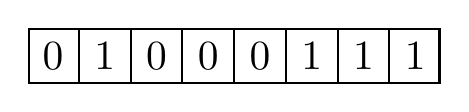
\begin{tikzpicture}[thick,scale=0.6, every node/.style={scale=1.5}]
\Byte {0, 1, 0, 0, 0, 1, 1, 1}
\end{tikzpicture}
\end{center}
\begin{enumerate}
\item What is the expected number of ones?
\item What is the expected value of the number represented by the resulting byte in decimal notation? In the example above, the number is $71$.
\end{enumerate}
\end{problem}
\begin{problem}
$A$ and $B$ pass the time by choosing numbers with distribution $U([0,1])$, for example on their computers, in rounds: first they each choose one number, then another, and so on. Without much knowledge of probability, they decide to check how often ``large'' numbers occur, say numbers greater than $0.75$. They choose two methods:
\begin{enumerate}
\item Each chooses 5 numbers, and they calculate the fraction of the 10 numbers that are greater than $0.75$.
\item As above, but each simulates 500 numbers.

Determine the average answers they would obtain under each procedure. What are the variances of the different methods? Which method would you choose, and why?
\item Over a large number of rounds, in what fraction of them will both numbers be greater than $0.75$? What is the expected number of rounds until at least one of the two numbers is greater than $0.75$?
\end{enumerate}
\begin{it}
Here is a sample realization:
\begin{center}
\begin{tabular}{l||l|l|l|l|l}
Round &1&2&3&4&5\\
$A$ &0.167&0.518&0.991&0.364&0.496\\
$B$ &0.296&0.840&0.755&0.143&0.646
\end{tabular}
\end{center}
The proportion in part 1 is $3/10$, the proportion in part 3 is $1/5$, and the number of rounds until at least one number exceeds $0.75$ is 2.
\end{it}
\end{problem}
\begin{problem}
A property near FMI costs EUR 250,000. An experienced estate agent can negotiate a different price, with the percentage change in the price being a random variable $X_1\sim N(-10,10)$. If you negotiate yourself, you can change the price by $X_2\sim N(0,100)$ percent, where $X_1$ and $X_2$ are independent.
\begin{enumerate}
\item What is the probability that the price is better if you negotiate yourself than if you use an agent?
\item What is the probability of negotiating a price below EUR 225,000 in each case?
\end{enumerate}
\end{problem}
\end{document}
